% =====================================================================
% Template Laporan Tugas — Workshop Deep Learning (Teknik Telekomunikasi ITERA)
% Studi Ablasi RNN, LSTM, GRU vs ANN untuk Prediksi Trafik Seluler
%
% Format IEEE conference dua kolom, MAKSIMAL 6 HALAMAN termasuk referensi.
% Compile: pdflatex main && bibtex main && pdflatex main && pdflatex main
%          (atau: latexmk -pdf main.tex). Bisa juga diunggah ke Overleaf.
%
% Teks bertanda [ ... ] adalah petunjuk: HAPUS dan ganti dengan isi kalian.
% =====================================================================
\documentclass[conference,a4paper]{IEEEtran}
\IEEEoverridecommandlockouts

\usepackage[indonesian]{babel}
\usepackage[utf8]{inputenc}
\usepackage[T1]{fontenc}
\usepackage{cite}
\usepackage{amsmath,amssymb}
\usepackage{graphicx}
\usepackage{booktabs}
\usepackage{siunitx}
\usepackage{xcolor}
\usepackage[hidelinks]{hyperref}
\graphicspath{{gambar/}}

% Penanda petunjuk (hapus pemakaiannya di versi akhir)
\newcommand{\petunjuk}[1]{\textcolor{gray}{[#1]}}

\begin{document}

\title{Studi Ablasi RNN, LSTM, dan GRU dibandingkan ANN untuk Prediksi Trafik Seluler Kota Milan}

% Satu blok per anggota (maks. 3). Hapus blok yang tidak dipakai.
\author{
\IEEEauthorblockN{Grasia Okta Adelia}
\IEEEauthorblockA{NIM 124400059\\
Teknik Telekomunikasi, ITERA\\
email@student.itera.ac.id}
\and
\IEEEauthorblockN{Egista Marga Kola}
\IEEEauthorblockA{NIM 124400003x\\
Teknik Telekomunikasi, ITERA\\
egista.124400003@student.itera.ac.id}
\and
\IEEEauthorblockN{Muhammad Allam Dzaky}
\IEEEauthorblockA{NIM 124400013\\
Teknik Telekomunikasi, ITERA\\
muhammad.124400013@student.itera.ac.id}
}

\maketitle

\begin{abstract}
\petunjuk{150--200 kata. Tuliskan: masalah (prediksi trafik internet per jam), data (Telecom Italia, kotak Duomo dan lokasi kelompok), apa yang diuji (ablasi faktor apa saja, 3 seed), temuan utama dengan angka (misalnya ``GRU terbaik dengan test MAE $x \pm y$, turun $z$\,\% dari acuan''), dan satu kalimat kesimpulan.}
\end{abstract}

\begin{IEEEkeywords}
prediksi trafik seluler, RNN, LSTM, GRU, studi ablasi
\end{IEEEkeywords}

% ---------------------------------------------------------------------
\section{Pendahuluan}
\petunjuk{Prediksi trafik seluler merupakan salah satu aspek penting
dalam pengelolaan jaringan telekomunikasi. Informasi mengenai
pola penggunaan jaringan dapat membantu operator memperkirakan
kebutuhan kapasitas, mengoptimalkan alokasi sumber daya, dan
menjaga kualitas layanan. Namun, trafik internet memiliki pola
yang berubah terhadap waktu sehingga diperlukan metode yang
mampu mempelajari hubungan temporal pada data.

Artificial Neural Network (ANN) dapat mempelajari hubungan
nonlinear antarfitur, tetapi tidak secara eksplisit memodelkan
urutan temporal seperti arsitektur rekuren. Recurrent Neural
Network (RNN) dirancang untuk memproses data berurutan,
sedangkan Long Short-Term Memory (LSTM) \cite{hochreiter1997lstm}
dan Gated Recurrent Unit (GRU) \cite{cho2014gru} menggunakan
mekanisme gerbang untuk membantu mempelajari dependensi temporal.
Meskipun demikian, kinerja setiap arsitektur juga dipengaruhi
oleh konfigurasi hiperparameter yang digunakan.

Penelitian ini membandingkan ANN, RNN, LSTM, dan GRU untuk
prediksi trafik internet per jam menggunakan data Telecom Italia
di Kota Milan. Studi ablasi dilakukan untuk mengevaluasi pengaruh
panjang jendela masukan, ukuran hidden, jumlah lapisan,
learning rate, dan kelompok fitur terhadap kinerja prediksi.
Konfigurasi model dievaluasi menggunakan beberapa seed agar
variasi hasil pelatihan dapat diamati.

Kontribusi penelitian ini meliputi: (1) perbandingan kinerja
empat arsitektur pada tugas prediksi trafik; (2) analisis
pengaruh hiperparameter dan fitur melalui eksperimen ablasi;
serta (3) evaluasi konfigurasi terbaik pada lokasi kelompok
untuk mengamati kemampuan generalisasi model.}

% ---------------------------------------------------------------------
\section{Data dan Metode}

\subsection{Dataset}
\petunjuk{Penelitian ini menggunakan dataset trafik jaringan seluler
dari Telecom Italia Big Data Challenge yang mencakup aktivitas
internet per jam di Kota Milan \cite{barlacchi2015milan}.
Data yang dianalisis meliputi trafik internet (\textit{net}),
panggilan (\textit{call}), dan SMS (\textit{sms}). Selain itu,
fitur waktu ditambahkan untuk merepresentasikan pola periodik
harian dan mingguan menggunakan transformasi sinus dan kosinus
pada jam serta hari dalam seminggu.

Eksperimen dilakukan pada lokasi Duomo sebagai lokasi acuan
dan lokasi kelompok, yaitu Stadio San Siro di Milan, dengan
kode lokasi 3 dan nomor kotak 5738. Data Duomo dibaca dari
berkas \texttt{milano\_duomo\_5060.csv}, sedangkan data lokasi
kelompok dibaca dari berkas \texttt{milano\_tugas\_10\_lokasi.csv}.
Penggunaan kedua lokasi tersebut memungkinkan perbandingan
kinerja model pada lokasi dengan karakteristik trafik yang
berbeda.}

\begin{figure}[t]
  \centering
  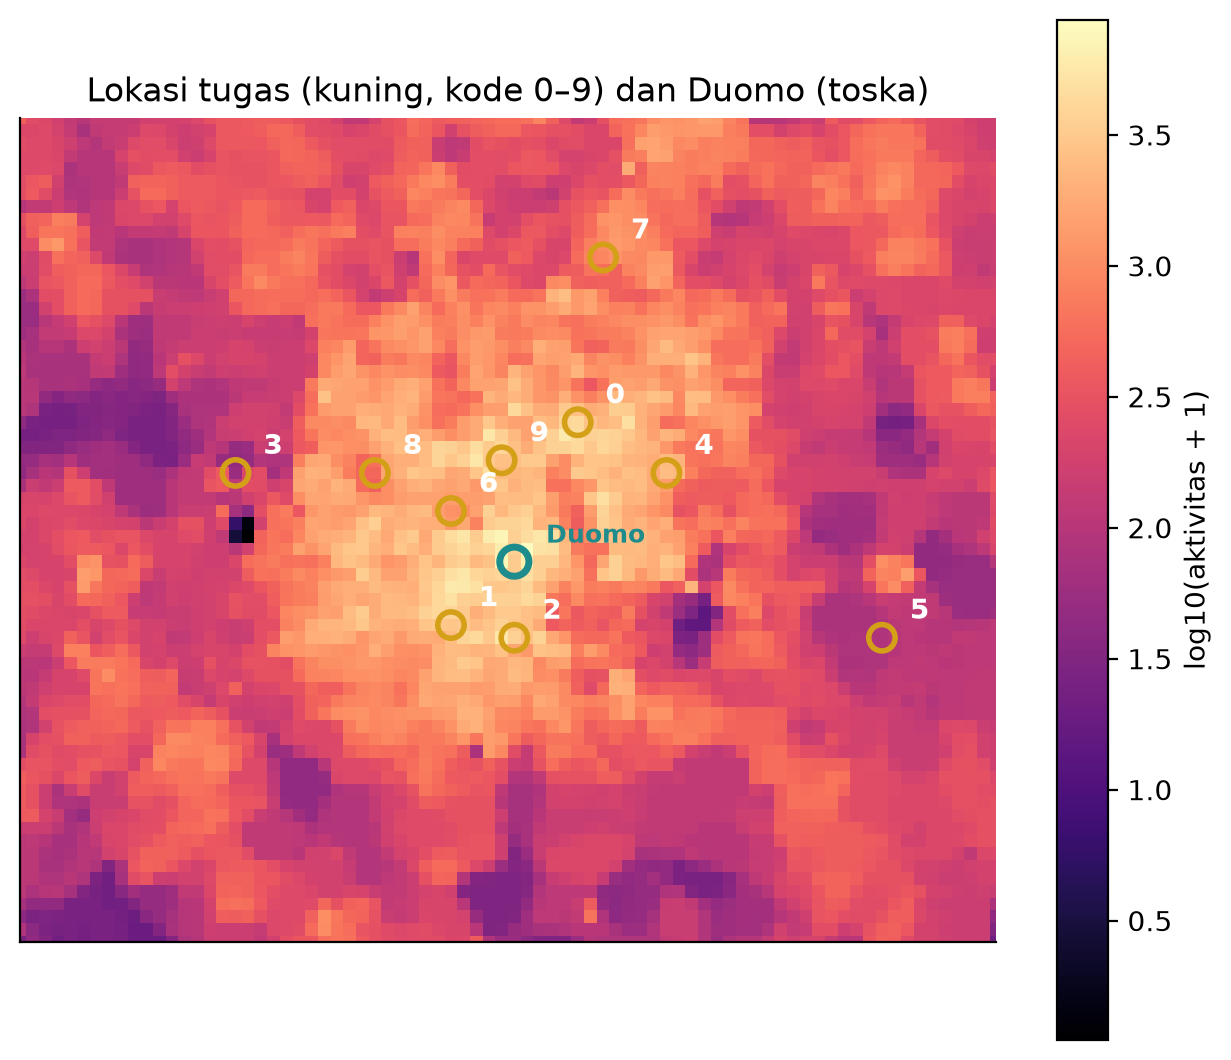
\includegraphics[width=0.85\linewidth]{peta_lokasi_tugas.png}
  \caption{Rata-rata aktivitas internet per kotak di Milan. Lingkaran kuning: lokasi tugas (kode 0--9); lingkaran toska: Duomo.}
  \label{fig:peta}
\end{figure}

\subsection{Pembagian Data dan Praproses}
\petunjuk{Dataset dibagi berdasarkan urutan waktu menjadi data
pelatihan (11 November--8 Desember 2013), validasi
(9--15 Desember 2013), pengujian (16--22 Desember 2013),
dan periode Natal mulai 23 Desember 2013 hingga akhir
data yang tersedia. Pembagian kronologis digunakan untuk
mempertahankan urutan temporal dan mencegah kebocoran
informasi dari masa depan ke proses pelatihan.

Sebelum digunakan, fitur distandarisasi menggunakan
rata-rata dan simpangan baku yang dihitung dari data
sebelum periode validasi. Selanjutnya, data dibentuk
menjadi jendela masukan sepanjang $W$ jam untuk
memprediksi trafik selama $H$ jam. Sampel dimasukkan
ke suatu subset berdasarkan waktu target terakhirnya,
sehingga evaluasi mengikuti periode yang telah ditentukan.}

\subsection{Model dan Konfigurasi Acuan}
\petunjuk{Penelitian ini membandingkan empat arsitektur jaringan saraf, yaitu Artificial Neural Network (ANN), Recurrent Neural Network (RNN), Long Short-Term Memory (LSTM), dan Gated Recurrent Unit (GRU). ANN digunakan sebagai model pembanding tanpa mekanisme rekuren, sedangkan RNN, LSTM, dan GRU digunakan untuk mempelajari pola temporal pada data trafik. Implementasi model disesuaikan dengan karakteristik masing-masing arsitektur.

Konfigurasi acuan menggunakan panjang jendela masukan sebesar 24 jam, horizon prediksi satu jam, seluruh kelompok fitur, dan ukuran batch 64. Pelatihan menggunakan optimizer Adam dengan *learning rate* sebesar 0,001 dan fungsi kerugian *mean squared error* (MSE). Nilai *dropout* ditetapkan sebesar 0, sedangkan jumlah epoch maksimum adalah 300 dengan *early stopping* berdasarkan kinerja validasi dan nilai *patience* sebesar 30.

Ukuran hidden dan jumlah lapisan ditetapkan berdasarkan arsitektur model. ANN menggunakan 32 unit hidden dengan dua lapisan, sedangkan RNN menggunakan 68 unit hidden, LSTM 33 unit hidden, dan GRU 38 unit hidden. Ketiga model rekuren tersebut masing-masing menggunakan satu lapisan. Konfigurasi ini digunakan sebagai acuan dalam eksperimen ablasi untuk mengamati pengaruh perubahan parameter terhadap kinerja prediksi.}

\begin{table}[t]
  \centering
  \caption{Konfigurasi acuan}
  \label{tab:acuan}
  \begin{tabular}{@{}ll@{}}
    \toprule
    Hyperparameter & Nilai acuan \\
    \midrule
    Panjang jendela $W$ & 24 jam \\
    Horizon & 1 jam \\
    Ukuran hidden & ANN 32, RNN 68, LSTM 33, GRU 38 \\
    Jumlah lapisan & ANN 2, rekuren 1 \\
    Fitur & net, call, sms, jam, hari (7) \\
    Optimizer, \textit{learning rate} & Adam, $10^{-3}$ \\
    \textit{Batch size} & 64 \\
    \textit{Early stopping} & \textit{patience} 30, maks.\ 300 epoch \\
    \bottomrule
  \end{tabular}
\end{table}

\subsection{Protokol Ablasi dan Evaluasi}
\petunjuk{Satu faktor diubah setiap kali; daftar faktor dan nilainya (A1--A5 dan dua faktor B pilihan kalian beserta hipotesis awal). Setiap konfigurasi dilatih dengan 3 seed; dilaporkan rata-rata $\pm$ simpangan baku. Metrik: MAE, RMSE, MAPE pada skala asli. Pemilihan konfigurasi terbaik memakai val MAE. Sebutkan perangkat yang dipakai (CPU/GPU) dan total waktu training.}

% ---------------------------------------------------------------------
\section{Hasil}

\subsection{Baseline Naif dan Acuan}
\petunjuk{Tabel baseline naif dan hasil konfigurasi acuan (Bagian 0).}

\subsection{Ablasi Wajib}
\petunjuk{Satu subbagian atau paragraf per faktor A1--A5. Gunakan grafik dari folder \texttt{hasil/} (boleh digabung beberapa dalam satu gambar agar hemat tempat) dan tabel seperti Tabel~\ref{tab:contoh}. Setiap gambar dan tabel harus dirujuk dan dibahas di teks.}

\begin{table}[t]
  \centering
  \caption{Contoh format: pengaruh panjang jendela $W$ terhadap test MAE (rata-rata $\pm$ simpangan baku, 3 seed). Angka di bawah hanya contoh.}
  \label{tab:contoh}
  \begin{tabular}{@{}lcccc@{}}
    \toprule
    $W$ (jam) & ANN & RNN & LSTM & GRU \\
    \midrule
    6   & $000 \pm 00$ & $000 \pm 00$ & $000 \pm 00$ & $000 \pm 00$ \\
    24  & $000 \pm 00$ & $\mathbf{000 \pm 00}$ & $000 \pm 00$ & $000 \pm 00$ \\
    168 & $000 \pm 00$ & $000 \pm 00$ & $000 \pm 00$ & $000 \pm 00$ \\
    \bottomrule
  \end{tabular}
\end{table}

\subsection{Ablasi Pilihan}
\petunjuk{Dua faktor B pilihan kalian: hipotesis awal, hasil, dan apakah hipotesis terbukti.}

\subsection{Konfigurasi Terbaik}
\petunjuk{Konfigurasi terbaik tiap model (dipilih dengan val MAE), lalu hasilnya pada minggu test dan Natal dibandingkan dengan acuan dan baseline naif.}

\subsection{Uji Generalisasi}
\petunjuk{Hasil acuan vs terbaik di lokasi kelompok. Apakah urutan model berubah? Kaitkan dengan pola trafik lokasi tersebut.}

% ---------------------------------------------------------------------
\section{Pembahasan}
\petunjuk{Bagian terpenting. Jangan hanya mengulang angka: jelaskan \emph{mengapa}. Hyperparameter mana yang paling berpengaruh dan mana yang tidak? Apakah perbedaan antar model lebih besar daripada perbedaan antar seed? Apa keterbatasan studi ini (satu kota, 4 minggu train, satu kali pembagian waktu)?}

% ---------------------------------------------------------------------
\section{Kesimpulan}
\petunjuk{3--5 kalimat yang menjawab pertanyaan studi, dengan angka.}

% ---------------------------------------------------------------------
\section*{Kontribusi Anggota}
\begin{tabular}{@{}lp{0.62\linewidth}@{}}
  Nama Anggota 1 & \petunjuk{contoh: Bagian A1--A3, penulisan Hasil} \\
  Nama Anggota 2 & \petunjuk{...} \\
  Nama Anggota 3 & \petunjuk{...} \\
\end{tabular}

\section*{Pernyataan Penggunaan AI}
\petunjuk{Tuliskan alat AI yang dipakai (misalnya ChatGPT, Claude, Copilot) dan untuk apa (memperbaiki kode, merapikan bahasa, dll.). Bila tidak memakai, tulis ``Tidak ada.'' Seluruh angka harus berasal dari run kalian sendiri.}

\section*{Kode dan Data}
Kode, notebook beserta output, dan seluruh hasil run tersedia di \url{https://github.com/username/nama-repo}.

\bibliographystyle{IEEEtran}
\bibliography{references}

\end{document}
